\documentclass[main.tex]{subfiles}
\begin{document}


\section{Middelwaardestellingen}
\label{sec:midd-van-rolle}

\subsection{Extrema}
\label{sec:extrema}

\begin{de}
  Beschouw een functie $f:\ A \subseteq \mathbb{R} \rightarrow \mathbb{R}$.
  We zeggen dat $f$ een \term{globaal maximum}, respectievelijk \term{globaal minimum} bereikt (over $A$) in een $a\in A$ als het volgende geldt:
  \[ \forall x\in A:\ f(a) \ge f(x) \quad\text{respectievelijk}\quad \forall x\in A:\ f(a) \le f(x)\]
\end{de}

\begin{de}
  Beschouw een functie $f:\ A \subseteq \mathbb{R} \rightarrow \mathbb{R}$.
  We zeggen dat $f$ een \term{lokaal maximum}, respectievelijk \term{lokaal minimum} bereikt (over $A$) in een $a\in A$ als het volgende geldt:
  \[ \exists \delta \in \mathbb{R}_{0}^{+}\forall x\in A:\ |x-a| < \delta \Rightarrow f(a) \ge f(x)\]
  respectievelijk
  \[ \exists \delta \in \mathbb{R}_{0}^{+}\forall x\in A:\ |x-a| < \delta \Rightarrow f(a) \le f(x)\]
\end{de}

\begin{de}
  Een \term{globaal extremum}, respectievelijk \term{lokaal extremum} is ofwel een globaal maximum ofwel een globaal minimum, respectievelijk ofwel een lokaal maximum ofwel een lokaal minimum.
\end{de}

\begin{de}
  \label{de:kritiek-punt}
  Een inwendig punt van een deel $A$ van $\mathbb{R}$ waarvoor $f'(a)=0$ geldt, noemt men een \term{kritiek punt} van $f$.
\end{de}

\begin{bpr}
  Beschouw een functie $f:\ A \subseteq \mathbb{R} \rightarrow \mathbb{R}$ en een inwendig punt $a$ van $A$.
  Stel dat $f$ een lokaal extremum bereikt in een $a$ en dat $f$ afleidbaar is in $a$, dan geldt $f'(a) = 0$, t.t.z dan is $a$ een kritiek punt van $f$.

  \begin{proof}
    Gevalsonderscheid:
    \begin{itemize}
    \item $f$ bereikt een lokaal maximum in $x$.
      Omdat $a$ een inwendig punt is van $A$ en een lokaal maximum bereikt in $a$ kunnen we een $\delta \in \mathbb{R}_{0}^{+}$ nemen als volgt:
      \[ \forall x\in \mathbb{R}: |x-a| < \delta \Rightarrow (x\in A \wedge f(a) \ge f(x)) \]
      Voor elke $h\in \mathbb{R}$ met $|h| < \delta$ zal $a+h$ dus tot $A$ behoren en ook het volgende gelden:
      \[ f(a+h) -f(a) \le 0 \]
      Beschouw nu de rij $(h_{n})_{n}$ gedefinieerd als volgt:
      \[ h_{n} = \frac{\delta}{2n} \]
      $(h_{n})_{n}$ convergeert dan naar $0$ maar geen enkele $h_{n}$ is nul.
      Bovendien geldt het volgende voor elke $n\in \mathbb{N}$:
      \[ \frac{f(a+h_{n}) -f(a)}{h_{n}} \le 0 \]
      Omdat de limiet de orde bewaart zal het volgende gelden:
      \[ f'(a) = \lim_{h\rightarrow 0}\frac{f(a+h)-f(a)}{h} = \lim_{n \rightarrow \infty}\frac{f(a+h_{n})-f(a)}{h_{n}} \le 0 \]
      Analoog vinden we dat $f'(a)$ ook groter dan of gelijk aan $0$ moet zijn:
      \[ \forall n\in \mathbb{N}:\ \frac{f(a-h_{n}) -f(a)}{h_{n}} \le 0 \]
      \[ f'(a) = \lim_{h\rightarrow 0}\frac{f(a-h)-f(a)}{h} = \lim_{n \rightarrow \infty}\frac{f(a-h_{n})-f(a)}{h_{n}} \ge 0 \]
      $f'(a)$ moet dus gelijk zijn aan $0$.
    \item $f$ bereikt een lokaal minimum in $x$.
      \extra{bewijs}
    \end{itemize}
  \end{proof}
\end{bpr}

\begin{tvb}
  Het omgekeerde van bovenstaande stelling geldt niet:
  Het beeld van een kritiek punt $a$ van een functie $f:\ A \subseteq \mathbb{R} \rightarrow \mathbb{R}$ is niet steeds een lokaal extremum.

  \begin{proof}
    \begin{figure}[H]
      \centering
      \begin{tikzpicture}[scale=.75]
        \begin{axis}[ymin=-2, ymax=2, xmin=-2, xmax=2]
          \addplot[smooth,domain=-2:2]{x^3};
        \end{axis}
      \end{tikzpicture}
    \end{figure}
    Beschouw de functie $f:\ \mathbb{R} \rightarrow \mathbb{R}:\ x \mapsto x^{3}$.
    De afgeleide functie $f'$ van $f$ ziet er als volgt uit:\vbref{vb:afgeleide-polynomiaal}
    \[ f':\ \mathbb{R} \rightarrow \mathbb{R}:\ x \mapsto 3x^{2} \]
    Het is duidelijk dat $f'$ nul is in $0$, maar ook dat $f(0)$ geen lokaal extremum is van $f$.
  \end{proof}
\end{tvb}

\subsection{Stijgen of dalen}
\label{sec:stijgen-dalen}

\begin{de}
  Beschouw een functie $f: J \subseteq \mathbb{R} \rightarrow \mathbb{R}$ gedefinieerd op een interval $J$.
  Zij $I$ een deelinterval van $J$.
  \begin{itemize}
  \item We zeggen dat $f$ \term{stijgt} als het volgende geldt.
    \[ \forall x,y \in I:\ x \le y \Rightarrow f(x) \le f(y) \]
  \item We zeggen dat $f$ \term{daalt} als het volgende geldt.
    \[ \forall x,y \in I:\ x \le y \Rightarrow f(x) \ge f(y) \]
  \item We zeggen dat $f$ \term{strikt stijgt} als het volgende geldt.
    \[ \forall x,y \in I:\ x < y \Rightarrow f(x) < f(y) \]
  \item We zeggen dat $f$ \term{strikt daalt} als het volgende geldt.
    \[ \forall x,y \in I:\ x < y \Rightarrow f(x) > f(y) \]
  \end{itemize}
\end{de}

\begin{bpr}
  Stel dat een functie $f: I \subseteq \mathbb{R} \rightarrow \mathbb{R}$ een afleidbare functie is op een open interval $I$.
  \begin{itemize}
  \item Als $f$ stijgt over $I$, dan geldt $\forall x\in I:\ f'(x) \ge 0$.
  \item Als $f$ daalt over $I$, dan geldt $\forall x\in I:\ f'(x) \ge 0$.
  \end{itemize}

  \begin{proof}
    Bewijs in delen.
    \begin{itemize}
    \item Zij $f$ een functie die stijgt over $I$.
      Kies nu een element $a$ van $I$.
      Omdat $I$ open is bestaat er een $\delta\in \mathbb{R}_{0}^{+}$ zodat voor alle $h<\delta$ $a+h$ tot $I$ behoort.
      Voor alle $h\in \mathbb{R}_{0}^{+}$ kleiner dan $\delta$ geldt nu het volgende:
      \[ \frac{f(a+h)-f(a)}{h} \ge 0 \]
      $a+h$ is immers groter dan, of gelijk aan, $a$ en $f$ is stijgend over $I$.
      De stelling volgt nu uit het feit dat limieten ongelijkheden behouden.\prref{pr:limiet behoudt ongelijkheid}
    \item 
      \extra{bewijs}
    \end{itemize}
  \end{proof}
\end{bpr}

\extra{het omgekeerde geldt ook} 

\subsection{Klassiekers}
\label{sec:twee-klassiekers}

\subsubsection{Rolle}
\label{sec:rolle}

\begin{bst}
  \label{st:rolle}
  De \term{middelwaardestelling van Rolle}\\
  Zij $f:\ \interval{a}{b} \rightarrow \mathbb{R}$ een continue functe op een begrensd gesloten interval $\interval{a}{b}$.
  Veronderstel dat $f$ afleidbaar is in $\interval[open]{a}{b}$ en dat $f(a)$ gelijk is aan $f(b)$.
  Er bestaat dan een $c\in \interval[open]{a}{b}$ zodat $f'(c)=0$ geldt.
  T.t.z. er bestaat dan een kritiek punt $c\in \interval[open]{a}{b}$.

  \begin{proof}
    Omdat $f$ een continue functie is, gedefinieerd op een gesloten begrensd interval, is $f$ begrensd.\needed
    De supremumeigenschap van $\mathbb{R}$ geeft ons dan dat er een supremum $M$ en een infimum $m$.
    \[ M = \sup\{f(x) \mid x \in \interval{a}{b} \} \]
    \[ m = \inf\{f(x) \mid x \in \interval{a}{b} \} \]
    \begin{itemize}
    \item
      Als $m$ gelijk is aan $M$, dan geldt $f(x)=f(a)$ voor alle $x \in \interval{a}{b}$ en is $f$ dus constant.
      In elke $c \in \interval{a}{b}$ is de afgeleide van $f$ dan nul.
    \item 
      Beschouw nu het geval dat $m< M$ geldt.
      Er treedt dan minstens \'e\'en van de volgende gevallen op:
      \begin{itemize}
      \item $f(a) < M$\\
        Er bestaat dan een $c$ zodat $f(c)$ gelijk is aan $M$.\stref{st:continue-functie-op-gesloten-begrensd-interval-bereikt-extrema}
        Omdat $f(a)$ gelijk is aan $f(b)$ en kleiner dan $M=f(c)$, kan $c$ niet gelijk zijn aan $a$ of aan $b$ en moet $c$ dus in het interval $\interval[open]{a}{b}$ liggen.
        $c$ is dan een kritiek punt, en dus is de afgeleide van $f$ in $c$ nul.\deref{kritiek-punt}
      \item $f(a) > m$\\
        \extra{bewijs}
      \end{itemize}
    \end{itemize}
  \end{proof}
\end{bst}

\begin{tvb}
  Bovenstaande stelling geldt niet in $\mathbb{Q}$.

  \begin{proof}
    Kies $f:\ \interval{0}{\sqrt{6}} \rightarrow \mathbb{Q}:\ x \mapsto \frac{x^{3}}{3}-2x$ zodat $f'(x) = x^{2}-2$.
    \begin{figure}[H]
      \centering
      \begin{tikzpicture}[scale=.75]
        \begin{axis}[ymin=-2, ymax=2, xmin=-0.1, xmax=2.5]
          \addplot[smooth,domain=0:2.4494]{((x^3)/3)-2*x};
          \addplot[soldot] coordinates{(0,0)(2.4494,0)};
          \addplot[holdot] coordinates{(1.4142,-1.8856)};
        \end{axis}
      \end{tikzpicture}
    \end{figure}
    $f(0)$ is gelijk aan $f(\sqrt{6})$ maar $f'$ heeft geen nulpunten in $\mathbb{Q}$.
\feed
  \end{proof}
\end{tvb}


\begin{st}
  Toepassinkje:\\
  Twee auto's rijden op een snelweg, in dezelde richting (en zin).
  Als de auto's op geen enkel tijdstip dezelfde snelheid hebben, dan kunnen de auto's elkaar hoogstens \'e\'en keer passeren.

  \begin{proof}
    Bewijs uit het ongerijmde: stel dat de auto's elkaar twee keer passeren.\\
    Noem de afstandsfunctie tussen de twee auto's $f$.
    Omdat de auto's elkaar twee keer passeren is geldt $f(a)=f(b)=0$ voor verschillende $a$ en $b$.
    Volgens de stelling van Rolle bestaat er dan een $c$ tussen $a$ en $b$ zodat $f'(c)$ nul is.
    Dit betekent dat de auto's op moment $c$ aan dezelfde snelheid reden.
    Contradictie.
  \end{proof}
\end{st}

\begin{st}
  Toepassingkje:\\
  De vergelijking $x^{3}+ax+b =0$ heeft precies \'e\'en oplossing.
  \begin{proof}
    In delen:
    \begin{itemize}
    \item Het aantal oplossingen is hoogstens \'e\'en:\\
      Uit het ongerijmde: stel dat er twee verschillende nulpunten bestaan van $x^{3}+ax+b$, dan bestaat er een $z$ tussen die nulpunten zodat $3z^{2} = -\frac{a}{3}$ geldt.
      Contradictie.
    \item Het aantal oplossingen is minstens \'e\'en:\\
\extra{bewijs}
    \end{itemize}
  \end{proof}
\end{st}

\subsubsection{Lagrange}
\label{sec:middelwaardestelling-lagrange}

\begin{bst}
  \label{st:middelwaardestelling-lagrange}
  De \term{middelwaardestelling van Lagrange}\\
  Zij $f:\ \interval{a}{b} \rightarrow \mathbb{R}$ een continue functe op een begrensd gesloten interval $\interval{a}{b}$.
  Veronderstel dat $f$ afleidbaar is in $\interval[open]{a}{b}$, dan bestaat er een $c\in \interval[open]{a}{b}$ als volgt.
  \[ f'(c) = \frac{f(b)-f(a)}{b-a} \]

  \begin{proof}
   Beschouw de hulpfunctie $g$:
   \[ g: \interval{a}{b} \rightarrow \mathbb{R}:\ x \mapsto g(x) = f(x)-\frac{f(b)-f(a)}{b-a}(x-a) \]
   In mensentaal uitgelegd is $g$ de functie die we bekomen als we de grafiek van $f$ draaien zodat de lijn tussen $(a,f(a))$ en $(b,f(b))$ horizontaal komt te liggen. (Dit is ook waarom het belangrijk is dat we $f$ op $\interval{a}{b}$ beschouwen, anders zou $g$ wel eens geen functie kunnen zijn.)
   \begin{itemize}
   \item $g$ is continu op $\interval{a}{b}$ want $g$ is opgebouwd uit continue functies.\vbref{vb:constante-functies-continu}\prref{pr:optelling-continu}\prref{pr:product-continu}\prref{pr:quotient-continu}
   \item Er geldt $g(a) = g(b)$:
     \[ g(a) = f(a)-\frac{f(b)-f(a)}{b-a}(a-a) = f(a) \]
     \[ g(b) = f(b)-\frac{f(b)-f(a)}{b-a}(b-a) = f(a) \]
     Er bestaat dus een $c\in \interval[open]{a}{b}$ zodat $g'(c)$ nul is.\stref{st:rolle}
   \item $g'$ ziet er bovendien als volgt uit: ($g$ is dus afleidbaar op $\interval[open]{a}{b}$.
     \[
     \begin{array}{rl}
       \lim_{x \rightarrow x}\frac{g(x)-g(a)}{x-a}
       &= \lim_{x \rightarrow a}\frac{f(x)-\frac{f(b)-f(a)}{b-a}(x-a) - f(a)}{x-a}\\
       &= \lim_{x \rightarrow a} \frac{f(x)-f(a)}{x-a} - \frac{f(b)-f(a)}{b-a}\\
       &= f'(x)-\frac{f(b)-f(a)}{b-a}\\
     \end{array}
     \]
   \item  In $c$ volgt uit $h'(c)$ de stelling:
     \[
     f'(c)-\frac{f(b)-f(a)}{b-a} = 0 
     \]
     \[
     f'(c) = \frac{f(b)-f(a)}{b-a} 
     \]
   \end{itemize}
  \end{proof}
\feed
\end{bst}


\begin{tvb}
  Bovenstaande stelling geldt niet in $\mathbb{Q}$.
  \begin{proof}
    Zie het tegenvoorbeeld voor de stelling van rolle.
  \end{proof}
\end{tvb}


\begin{de}
  Zij $f:\mathbb{R} \rightarrow \mathbb{R}$ een afleidbare functie.
  Een vast punt $x \in \mathbb{R}$ is een punt waarvoor $f(x) = x$ geldt.
\end{de}

\begin{st}
  \label{st:vast-punt-uniek-voor-specifieke-functie}
  Zij $f:\mathbb{R} \rightarrow \mathbb{R}$ een afleidbare functie met de volgende eigenschap, dan heeft $f$ hoogstens \'e\'en vast punt.
  \[ \forall t\in \mathbb{R}: f'(t) \neq 1 \]
  
  \begin{proof}
    Bewijs uit het ongerijmde: Stel dat $f$ minstens twee vaste punten heeft.\\
    Noem $v$ en $w$ de vaste punten van $f$.
    De middelwaardestelling van Lagrange geeft ons dan een $c$ zodat $f'(c)$ gelijk is aan $\frac{v-w}{v-w} = 1$. contradictie.
  \end{proof}
\end{st}

\begin{st}
  Zij $f:\mathbb{R} \rightarrow \mathbb{R}$ een afleidbare functie met de volgende eigenschap, dan heeft $f$ precies \'e\'en vast punt.
  \[ \exists A \in \interval[open right]{0}{1}:\ \forall t \in \mathbb{R}:\ |f'(t)| \le A \]
  Het vast punt wordt bovendien gegeven als de volgende limiet:
  \[ \lim_{n \rightarrow +\infty}x_{n} \text{ met } x_{n+1} = f(x_{n}) \text{ en } x_{0} \text{ willekeurig.} \]

  \begin{proof}
    We weten al dat als $f$ een vast punt heeft dat dat vast punt dan uniek is.\stref{st:vast-punt-uniek-voor-specifieke-functie}
    \extra{bewijs daat die limiet een vast punt is.}
  \end{proof}
\end{st}


\subsubsection{Cauchy}
\label{sec:cauchy}

\begin{bst}
  \label{st:middelwaardestelling-cauchy}
  De \term{middelwaardestelling van Cauchy}\\
  Zij $f,g:\ \interval{a}{b} \rightarrow \mathbb{R}$ continue functes op een begrensd gesloten interval $\interval{a}{b}$.
  Veronderstel dat $f$ en $g$ afleidbaar zijn in $\interval[open]{a}{b}$, dan bestaat er een $c\in \interval[open]{a}{b}$ als volgt.
  \[ \left( f(b) - f(a) \right) g'(c) = f'(c) \left( g(b) - g(a) \right) \]

  \begin{proof}
    Beschouw de hulpfunctie $h$:
    \[ h:\ \interval{a}{b} \rightarrow \mathbb{R}:\ x \mapsto h(x) = (f(b)-f(a))g(x) -f(x)(g(b)-g(a)) \]
    \begin{itemize}
    \item $h$ is continu op $\interval{a}{b}$ want zowel $f$ als $g$ is continu op $\interval{a}{b}$.
    \item Er geldt $h(a)=h(b)$:
      \[
      \begin{array}{rl}
        h(a) &= (f(b)-f(a))g(a) -f(a)(g(b)-g(a))\\
             &= f(b)g(a)-f(a)g(a)-f(a)g(b)+f(a)g(a)\\
             &= f(b)g(a)-f(a)g(b)
      \end{array}
      \]
      \[
      \begin{array}{rl}
        h(b) &= (f(b)-f(a))g(b) -f(b)(g(b)-g(a))\\
             &= f(b)g(b)-f(a)g(b) -f(b)g(b)+f(b)g(a)\\
             &= f(b)g(a)-f(a)g(b)
      \end{array}
      \]
     Er bestaat dus een $c\in \interval[open]{a}{b}$ zodat $h'(c)$ nul is.\stref{st:rolle}
    \item $h'$ ziet er bovendien als volgt uit:
      \[
      h'(x) = (f(b)-f(a))g'(x)-f'(x)(g(b)-g(a))
      \]
   \item In $c$ volgt uit $h'(c)$ de stelling:
     \[
     (f(b)-f(a))g'(c)-f'(c)(g(b)-g(a)) = 0
     \]
     \[
     (f(b)-f(a))g'(c) = f'(c)(g(b)-g(a))
     \]
    \end{itemize}
  \end{proof}
  \feed
\end{bst}

\begin{st}
  Zij $f:\ \mathbb{R} \rightarrow \mathbb{R}$ een functie die afleidbaar over $\mathbb{R} \setminus \{c\}$ zodat $\lim_{x\rightarrow c}f'(x)$ bestaat en eindig is, dan is $f$ afleidbaar in $c$.
\extra{bewijs}
\end{st}

\subsection{Stijgen, dalen of constant zijn}

\begin{bpr}
  Zij $f:\ \interval{a}{b} \rightarrow \mathbb{R}$ een continue functe op een begrensd gesloten interval $\interval{a}{b}$ die afleidbaar is in $\interval[open]{a}{b}$.
  \begin{itemize}
  \item Als $f'(c) \ge 0$ geldt voor alle $c \in \interval[open]{a}{b}$, dan is $f$ stijgend in $\interval{a}{b}$
    \[ \forall x,y \in \interval{a}{b}:\ x \le y \Rightarrow f(x) \le f(y) \]
  \item Als $f'(c) \le 0$ geldt voor alle $c \in \interval[open]{a}{b}$, dan is $f$ dalend in $\interval{a}{b}$
    \[ \forall x,y \in \interval{a}{b}:\ x \le y \Rightarrow f(x) \ge f(y) \]
  \end{itemize}

  \begin{proof}
    Elk deel appart.
    \begin{itemize}
    \item Kies willekeurig $x$ en $y \in \interval{a}{b}$ met $x\le y$.
      We passen de middelwaardestelling van lagrange toe op de functie $f$, beperkt tot het interval $\interval{x}{y}$.\stref{st:middelwaardestelling-lagrange}
      Dit levert een $c\in \interval[open]{x}{y}$ als volgt:
      \[ f(y)-f(x) = f'(c)(y-x) \]
      Omdat $f'(c)$ positief is, alsook $(y-x)$, geldt $f(y)-f(x) \ge 0 \Leftrightarrow f(y) \ge f(x)$.
    \item \extra{bewijs}
    \end{itemize}
  \end{proof}
\end{bpr}

\begin{bpr}
  Zij $f:\ \interval{a}{b} \rightarrow \mathbb{R}$ een continue functe op een begrensd, gesloten interval $\interval{a}{b}$ die afleidbaar is in $\interval[open]{a}{b}$.
  Als $\forall c\in \interval[open]{a}{b}: f'(c) = 0$ geldt, dan is $f$ constant.

  \begin{proof}
    Kies willekeurig een $x\in \interval[open left]{a}{b}$.\clarify{waarom halfopen?}
    We passsen de middelwaardestelling van Lagrange toe op de functie $f$, beperkt tot het interval $\interval{a}{x}$.\stref{st:middelwaardestelling-lagrange}
    Dit levert een $c\in \interval[open]{a}{x}$ als volgt:
    \[ f(x)-f(a) = f'(c)(x-a) \]
    Omdat $f'(c)$ nul is, moet $f(x)$ gelijk zijn aan $f(a)$.
  \end{proof}
\extra{rechtstreeks bewijzen vanuit de definitie van een afgeleide}
\end{bpr}

\begin{tvb}
  Bovenstaande stelling geldt niet wanneer we het interval $\interval{a}{b}$ vervangen door een willekeurig deel $A$ en $\interval[open]{a}{b}$ door $\mathring{A}$.
  \begin{proof}
    Beschouw de functie $f$ als volgt. $f$ is overal afleidbaar op zijn domein en de afgeleide is overal $0$, maar $f$ is niet constant.
    \[
    f:\ \interval[open]{0}{1}\cup \interval[open]{2}{3}:\ x \mapsto
    \left\{
      \begin{array}{rl}
        0 & \text{ als } x \in \interval[open]{0}{1}\\
        1 & \text{ als } x \in \interval[open]{2}{3}
      \end{array}
    \right.
    \]
    \begin{figure}[H]
      \centering
      \begin{tikzpicture}[scale=.75]
        \begin{axis}[ymin=-1.1, ymax=2.1, xmin=-0.3, xmax=3.3]
          \addplot[smooth,domain=0:1]{0};
          \addplot[smooth,domain=2:3]{1}; \addplot[holdot]
          coordinates{(0,0)(1,0)(2,1)(3,1)};
        \end{axis}
      \end{tikzpicture}
    \end{figure}
  \end{proof}
\end{tvb}
\extra{tegenvoorbeelden voor de interval-heid voorwaarde op $A$?}

\begin{gst}
  Zij $f:\ \mathbb{R} \rightarrow \mathbb{R}$ een functie die afleidbaar is in een punt $a\in \mathbb{R}$ met $f'(a) \ge 0$.
  Het is niet waar dat er een open interval rond $a$ bestaat zodat $f$ stijgt over dat interval.
\extra{vind een tegenvoorbeeld hint: rare sinus!}
\end{gst}

\subsection{Limieten van rijen van afleidbare functies}
\label{sec:limieten-van-rijen}

\begin{bst}
  Beschouw een rij $(f_{n})_{n}$ van afleidbare functies gedefinieerd op een interval $I \subseteq \mathbb{R}$ met waarden in $\mathbb{R}$.
  Stel dat $(f_{n})_{n}$ puntsgewijs convergeert naar een functie $f:\ I \rightarrow \mathbb{R}$ en dat $(f'_{n})_{n}$ uniform op $I$ convergeert, dan is $f$ afleidbaar:
  \[ \forall a\in I:\ f'(a) = \lim_{n\rightarrow +\infty}f_{n}'(a) \]

  \begin{proof}
    We tonen het volgende aan:
    \[ \forall a\in I:\ \lim_{x\rightarrow a}\frac{f(x)-f(a)}{x-a} = \lim_{n\rightarrow +\infty}f_{n}'(a) \]
    Noem het rechterlid $L$.
    \begin{itemize}
    \item Merk eerst op dat voor alle $x\in I$, verschillend van $a$, en alle $m\in \mathbb{N}$ het volgende geldt:
      \[
      \begin{array}{rl}
        \left| \frac{f(x)-f(a)}{x-a} - L \right| 
        &\le \left| \frac{f(x)-f(a)}{x-a} - \frac{f_{m}(x)-f_{m}(a)}{x-a} \right|\\
        &+ \left| \frac{f_{m}(x)-f_{m}(a)}{x-a} - f_{m}'(a) \right|\\
        &+ \left| f'_{m}(a) - L \right|
      \end{array}
      \]
    \item Kies nu een willekeurige $\epsilon \in \mathbb{R}_{0}^{+}$.
      \begin{itemize}
      \item 
        Omdat $(f_{n}')_{n}$ uniform convergeert naar $f'(x)$ (moet het een Cauchyrij zijn \waarom en ) kunnen we een $n_{0}\in \mathbb{N}$ vinden als volgt:
        \[ \forall m,n \ge n_{0},\forall y\in I:\ |f'_{n}(y)-f'_{m}(y)| < \frac{\epsilon}{3} \]
        Vanwege de middelwaardestelling van lagrange bestaat er voor elke $x\in I$, verschillend van $a$, en voor elke $n,m\in \mathbb{N}$ een $c$ tusen $a$ en $x$ als volgt:\stref{st:middelwaardestelling-lagrange}
        \[ \left| \frac{f_{n}(x)-f_{n}(a)}{x-a} - \frac{f_{m}(x)-f_{m}(a)}{x-a}\right| = \left| f'_{n}(c) -f'_{m}(c) \right| \]
        We vinden dus het volgende:
        \[ \forall m,n \ge n_{0},\forall y\in I:\ \left| \frac{f_{n}(x)-f_{n}(a)}{x-a} - \frac{f_{m}(x)-f_{m}(a)}{x-a}\right| < \frac{\epsilon}{3} \]
        Nemen we hiervan de limiet voor $n$ gaande naar $+\infty$, dan vinden we de volgende ongelijkheid.
        \[ \forall m \ge n_{0},\forall y\in I:\ \left| \frac{f(x)-f(a)}{x-a} - \frac{f_{m}(x)-f_{m}(a)}{x-a}\right| \le \frac{\epsilon}{3} \]
        \clarify{waarom plots $\le$?}
      \item 
        Omdat $f'_{n}(a)$ uniform naar $L$ convergeert, kunnen we een $m_{0} \in \mathbb{N}$ vinden zodat het volgende geldt:
        \[ \forall m\in \mathbb{N}: m \ge m_{0} \Rightarrow \left| f'_{m}(a) - L \right| < \frac{\epsilon}{3}\]
      \item 
        Omdat $f_{m}$ afleidbaar is in $a$, kunnnen we een $\delta \in \mathbb{R}_{0}^{+}$ vinden  als volgt:
        \[ \forall x\in I: 0 < |x-a| < \delta:\ \left| \frac{f_{m}(x)-f_{m}(a)}{x-a} - f_{m}'(a) \right| < \frac{\epsilon}{3} \]
      \end{itemize}
    \item Uit het eerste puntje volgt nu de stelling:
      \[ \forall x\in I:\ 0 < |x-a| < \delta:\ \left| \frac{f(x)-f(a)}{x-a} - L \right|  < \frac{\epsilon}{3}+\frac{\epsilon}{3} +\frac{\epsilon}{3} = \epsilon \]
    \end{itemize}
  \end{proof}
\end{bst}

\begin{tvb}
  Bovenstaande functie geldt niet als $(f'_{n})_{n}$ niet uniforum convergeert naar $f'_{n}$.
  \begin{proof}
    Beschouw de volgende rij afleidbare functies $f_{n}$.

    \noindent
    \begin{minipage}{.45\textwidth}
    \begin{figure}[H]
      \centering
      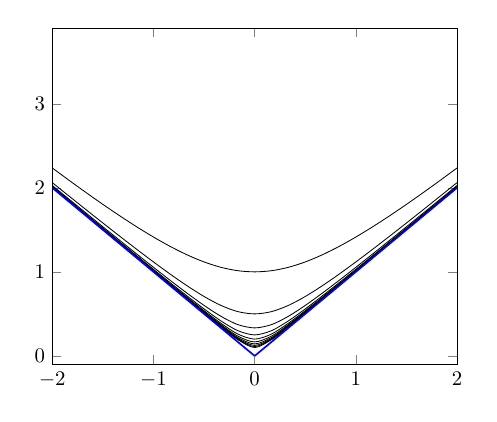
\begin{tikzpicture}[scale=.75]
        \begin{axis}[xmin=-2, xmax=2,ymin=-0.1, ymax=3.9]
          \foreach \n in {1,...,10}{
            \addplot[smooth,domain=-2:2]{sqrt(x^2+(1/\n^2))};
          }
          \addplot[smooth,color=blue,thick,domain=-2:0]{-x};
          \addplot[smooth,color=blue,thick,domain=0:2]{x};
        \end{axis}
      \end{tikzpicture}
    \end{figure}
    \end{minipage}
    \begin{minipage}{.45\textwidth}
    \[ f_{n}:\ \mathbb{R} \rightarrow \mathbb{R}:\ x \mapsto \sqrt{x^{2}+ \frac{1}{n^{2}}} \]
    \[ f:\ \mathbb{R} \rightarrow \mathbb{R}:\ |x| \]
    \end{minipage}
    Voor elke $x\in \mathbb{R}$ geldt $\lim_{n\rightarrow \infty}f_{n}(x) = \sqrt{x^{2}} = |x|$, dus de rij functies convergeert al zeker puntsgewijs naar $f$.
    De convergentie is bovendien uniforum op $\mathbb{R}$ vanwege de volgende afschatting:
    \[
    \left| \sqrt{x^{2}+\frac{1}{n^{2}}} - |x| \right|
    = \frac{\frac{1}{n^{2}}}{\sqrt{x^{2}+\frac{1}{n^{2}}} + |x|}
    \le \frac{1}{n^{2}}
    = \frac{1}{n}
    \]
\extra{uitwerken?}
    We hebben nu een rij afleidbare functies $(f_{n})_{n}$ die uniforum convergeert op $\mathbb{R}$ naar een functie $f$ die niet afleidbaar is in $0$.
    $(f_{n}')_{n}$ convergeert dus niet naar $f'$.
  \end{proof}
\end{tvb}

\subsection{De regel van de l'H\^opital}
\label{sec:de-regel-van}

\begin{bpr}
  Beschouw functies $f,g:\ A \subseteq \mathbb{R} \rightarrow \mathbb{R}$ en een $a\in A$ die een ophopingspunt is van $A$.
  Stel dat $f(a)=g(a)=0$ geldt, dan $f$ en $g$ afleidbaar zijn in $a$ en dat $g'(a)$ niet nul is, dan bestaat $\lim_{x \rightarrow a}\frac{f(x)}{g(x)}$ en geldt:
  \[ \lim_{x\rightarrow a}\frac{f}{g}= \frac{f'(a)}{g'(a)} \]

  \begin{proof}
    \[
    \begin{array}{rl}
      \frac{f'(a)}{g'(a)}
      &= \frac{\lim_{x\rightarrow a}\frac{f(x)-f(a)}{x-a}}{\lim_{x\rightarrow a}\frac{g(x)-g(a)}{x-a}}\\
      &= \lim_{x\rightarrow a}\frac{\frac{f(x)-f(a)}{x-a}}{\frac{g(x)-g(a)}{x-a}}\\
      &= \lim_{x\rightarrow a}\frac{f(x)-f(a)}{g(x)-g(a)}\\
      &= \lim_{x\rightarrow a}\frac{f}{g}
    \end{array}
    \]
    We gebruiken in de tweede gelijkheid dat $g'(a)$ niet nul is.\prref{pr:limiet-door-quotient}
  \end{proof}
\end{bpr}

\begin{st}
  De \term{regel van de l'H\^opital}\\
  Beschouw functies $f,g:\ I \subseteq \mathbb{R} \rightarrow \mathbb{R}$, gedefinieerd op een interval $I$.
  Zij $a\in \mathbb{R} \cup \{-\infty,+\infty\}$ een ophopingspunt van $I$.
  Stel dat $f$ en $g$ afleidbaar zijn in $I \setminus \{a\}$ en dat $g(x)$ en $g'(x)$ beide niet nul zijn voor alle $I \setminus \{a\}$.
  Stel dat $\lim_{x\rightarrow a}f(x)$ en $\lim_{x\rightarrow a}g(x)$ beide nul zijn of dat $\lim_{x\rightarrow a}g(x) = \pm\infty$ geldt.
  \begin{center}
    Als $\lim_{x\rightarrow a}\frac{f'(x)}{f'(a)}$ bestaat, dan bestaat ook $\lim_{x\rightarrow a}\frac{f(x)}{f(a)}$ en zijn ze gelijk.
  \end{center}

  \begin{proof}
    Groot gevalsonderscheid:
    We onderscheiden alle (27) gevallen in
    \[
    \left\{ a \in \mathbb{R}, a = +\infty, a = -\infty \right\}
    \]\[\times\]\[
    \left\{ \lim_{x\rightarrow a}f(x) = \lim_{x\rightarrow a}g(x) = 0, \lim_{x\rightarrow a}g(x) =-\infty ,\lim_{x\rightarrow a}g(x) =+\infty  \right\}
    \]\[\times\]\[
    \left\{ \lim_{x\rightarrow a}\frac{f'(x)}{f'(a)} = L \in \mathbb{R}, \lim_{x\rightarrow a}\frac{f'(x)}{f'(a)} = +\infty, \lim_{x\rightarrow a}\frac{f'(x)}{f'(a)} = -\infty \right\}
    \]

    \begin{itemize}
    \item $a\in \mathbb{R}$, $\lim_{x\rightarrow a}f(x) = \lim_{x\rightarrow a}g(x) = 0$ en $\lim_{x\rightarrow a}\frac{f'(x)}{f'(a)} = L \in \mathbb{R}$.\\
      We zullen bewijzen dat $\lim_{x\rightarrow a}\frac{f(x)}{f(a)}$ gelijk is aan $L$.
      Kies daartoe een willekeurige $\epsilon \in \mathbb{R}_{0}^{+}$.
      Omdat $\lim_{x \rightarrow a}\frac{f'(x)}{f'(a)} = L$ geldt, kunnen we een $\delta \in \mathbb{R}_{0}^{+}$ vinden als volgt:
      \[ \forall c\in I:\ 0<|c-a|<\delta \Rightarrow \left|\frac{f'(c)}{g'(c)}-L\right| < \epsilon \]
      Kies nu een willekeurige $x\in I$ met $0<|x-a|< \delta$, groter dan $a$ (het andere geval is analoog).
      Merk op dat $\interval[open]{a}{x}$ nu een deel is van $I$ en dat $\forall y \in \interval[open]{a}{x}: g(x)\neq g(y)$ geldt.
      (Er zou anders immers een punt $c$ tussen $x$ en $y$ liggen met $g'(c) =0$\stref{st:rolle} en we namen aan van niet.)
      Kies een willekeurige $y \in \interval[open]{a}{x}$, en merk nu eerst nog het volgende op:
      \[ \frac{f(x)}{g(x)} = \frac{f(x)-f(y)}{g(x)-g(y)}\frac{g(x)-g(y)}{g(x)} + \frac{f(y)}{g(y)} \]
      Omdat $\lim_{y \rightarrow a}g(y)$ nul is, geldt het volgende
      \[ \lim_{y \rightarrow a}\frac{g(x)-g(y)}{g(x)} = \frac{g(x)}{g(x)} = 1 \]
      Omdat $\lim_{y\rightarrow a}(y)$ en $\lim_{y \rightarrow a}g(y)$ beide nul zijn geldt ook het volgende:
      \[ \lim_{y \rightarrow a}\frac{f(y)}{g(x)} = \frac{0}{g(x)} = 0 \]
      We kunnen nu de limiet nemen voor $y$ gaande naar $a$ van de opmerking:
      \[
      \begin{array}{rl}
        \frac{f(x)}{g(x)}
        &= \lim_{y \rightarrow a}\left(\frac{f(x)-f(y)}{g(x)-g(y)}\frac{g(x)-g(y)}{g(x)} + \frac{f(y)}{g(y)}\right)\\
        &= \lim_{y \rightarrow a}\frac{f(x)-f(y)}{g(x)-g(y)}\lim_{y \rightarrow a}\frac{g(x)-g(y)}{g(x)} + \lim_{y \rightarrow a}\frac{f(y)}{g(y)}\\
        &= \lim_{y \rightarrow a}\frac{f(x)-f(y)}{g(x)-g(y)} \cdot 1 + 0\\
        &= \lim_{y \rightarrow a}\frac{f(x)-f(y)}{g(x)-g(y)}\\
      \end{array}
      \]
      Er bestaat een $c\in \interval[open]{x}{y}$ als volgt:\stref{st:middelwaardestelling-cauchy}
      \question{de stelling van Cauchy geldt voor continue functies op een gesloten en begrensd interval, dit is open?!}
      \[ \left( f(b) - f(a) \right) g'(c) = f'(c) \left( g(b) - g(a) \right) \]
      Voor die $c$ geldt dan het volgende:
      \[ \frac{f(x)-f(y)}{f(x)-g(y)} = \frac{f'(c)}{g'(c)} \]
      Omdat $c$ tussen $x$ en $y$ lag, $y$ tussen $a$ en $x$, en $x$ tussen $a$ en $a+\delta$, ligt $c$ ook tussen $a$ en $a+\delta$.
      Er geldt dus het volgende voor $c$:
      \[ \left|\frac{f(x)-f(y)}{g(x)-g(y)} - L\right| = \left| \frac{f'(c)}{g'(c)} - L \right| < \epsilon \]
      We vinden zo dat $L$ de limiet is van $\frac{f(x)}{f(a)}$ voor $x$ gaande naar $a$:
      \[ \left|\frac{f(x)}{f(a)}-L\right| = \left|\lim_{y \rightarrow a}\frac{f(x)-f(y)}{g(x)-g(y)} - L \right| = \left| \lim_{y\rightarrow a}\frac{f'(c)}{g'(c)} - L \right| < \epsilon \]
\extra{uitleg uitschrijven voor het bewijs want ik snap er precies nog niets van.}
    \end{itemize}
\extra{al de rest}
  \end{proof}
\end{st}



\subsection{Een tussenwaardestelling voor afgeleide}
\label{sec:een-tuss-voor}


\begin{bst}
  Beschouw een afleidbare functie $f:\ I \rightarrow \mathbb{R}$, gedefinieerd op een interval $I \subseteq \mathbb{R}$.
  Noem $x_{1},x_{2} \in I$ met $x_{1}< x_{2}$ waarvoor $f'(x_{1}) \neq f'(x_{2})$ en $y\in \mathbb{R}$ zodat $y$ tussen $f'(x_{1})$ en $f'(x_{2})$ ligt.
  Er bestaat dan een $x \in \interval[open]{x_{1}}{x_{2}}$ waarvoor $f'(x) = y$ geldt.
\TODO{bewijs p 34}
\end{bst}

\begin{gev}
  De afgeleide functie van een afleidbare functie $f:\ I \rightarrow \mathbb{R}$, gedefinieerd op een interval $I \subseteq \mathbb{R}$ kan geen discontinu\"iteiten van de eerste soort bevaten.
\TODO{bewijs p 34}
\end{gev}





\end{document}

%%% Local Variables:
%%% mode: latex
%%% TeX-master: t
%%% End:
